\documentclass[twocolumn]{IEEEtran}
\usepackage[utf8x]{inputenc}
\usepackage{amssymb,amsfonts}
\usepackage[tbtags]{amsmath}
\usepackage{graphicx}
\usepackage{cite}
\usepackage{slashbox}
\usepackage{pict2e}
\usepackage{float}
\usepackage[all]{xy}
\usepackage{graphics,graphicx,color,colortbl}
\usepackage{times}
\usepackage{subfigure}
\usepackage{wrapfig}
\usepackage{multicol}
\usepackage{cite}
\usepackage{url}
\usepackage[tbtags]{amsmath}
\usepackage{amsmath,amssymb,amsfonts,amsbsy}
\usepackage{bm}
\usepackage{algorithm}
\usepackage{algorithmic}
\usepackage[centerlast, small]{caption}
\usepackage[colorlinks=true, citecolor=blue, linkcolor=blue, urlcolor=blue,
breaklinks=true]{hyperref}

\begin{document}
\title{Circuitos Trifásicos}
\author{José Fabio Lozano Ovalle Código: $222982$\\
	Wilson Orlando Macias Fuquen Código: $223101$\\
	David Ricardo Martínez Hernández Código: $261931$}
\maketitle
\markboth{Universidad Nacional de Colombia}{}
\floatname{algorithm}{Algoritmo}

\begin{abstract}
Se construirán cargas trifásicas balanceadas en estrella y delta  que  se alimentaran con fuentes trifásicas balanceadas  y se analizan los voltajes y corrientes de línea y fase, también  se realizaran los diagramas fasoriales. Se construirá un circuito rectificador trifásico de media onda y por ultimo se medirán las potencias activa reactiva y aparente tanto monofásica como trifásica.
\end{abstract}

\begin{keywords}
Cargas Balanceadas, Conexión Estrella (Y), Conexión Triangulo ($\Delta$), Corriente de Fase, Corriente de Línea, Neutro, Potencia Activa, Potencia Aparente, Potencia Reactiva, Voltaje de Fase, Voltaje de Línea.
\end{keywords}

\section{Objetivos}
\begin{itemize}
 \item Identificar la relación entre voltajes fase-fase y voltajes fase-neutro en un sistema trifásico para cargas en estrella y en delta.
 \item Identificar la relación entre la corriente fase-fase y la corriente fase-neutro en un sistema trifásico para cargas en estrella y en delta.
 \item Utilizar el método de los dos watimetros “ARON” para la medición de potencia.
 \item Determinar la variación de la potencia cuando se implementa un rectificador de media onda.
\end{itemize}

\section{Introducción}
\noindent
La mayor parte del equipo utilizado en nuestra vida cotidiana funciona con sistemas monofásicos, pero existen muchos otros que utilizan el sistema trifásico, como por ejemplo los motores en la industria, y que representan una gran parte de la demanda total del sistema.\\
La utilización de circuitos trifásicos para la generación de energía eléctrica presenta  ventajas no solo desde el punto de vista constructivo de la maquina rotatoria que se utiliza para dicha generación, sino también para la transmisión de potencia, ya que la eficiencia mejora cuando se utiliza un sistema trifásico en vez de uno monofásico. La potencia instantánea de la carga se mantiene como una constante lo cual ayuda a mantener también constante el momento de torsión sobre el rotor, esto no seria posible en un sistema monofásico y se traduciría en un aumento en la vibración del generador.

\section{Hipótesis}
\noindent
Al medir la potencia con el método de los dos watimetros la suma de la potencia activa registrada por cada uno será la potencia trifásica total que consume la carga.\\
Los voltajes de línea serán mayores en una magnitud de $\sqrt{3}$ a los voltajes de fase en una conexión estrella-estrella (Y-Y).\\
Las corrientes de línea serán mayores en una magnitud de $\sqrt{3}$ a las corrientes de fase en una conexión estrella-delta (Y-$\Delta$).

\section{Actividades a Desarrollar en el Laboratorio}
\noindent
\begin{itemize}
 \item Se identifico el neutro de la red monofásica midiendo la diferencia de potencial entre los terminales con respecto a tierra, el que diera aproximadamente $0$ es el neutro que se necesita.
 \item En el segundo punto se midieron Voltajes, Corrientes y Potencias del circuito Y-Y balanceado. De igual forma se realizo este procedimiento para el circuito Y-$\Delta$ balanceado.
\end{itemize}


\section{Análisis y Resultados}
\noindent
Para esta práctica se implementaran tres circuitos trifásicos con fuentes balanceadas, a continuación se muestran los montajes de estos.

\subsection{Circuito $Y-Y$}
\noindent
Para esta parte de la práctica se implementa el siguiente circuito trifásico $Y-Y$ con cargas balanceadas para el cual se hace el análisis correspondiente.
\begin{figure}[H]
	\centering
		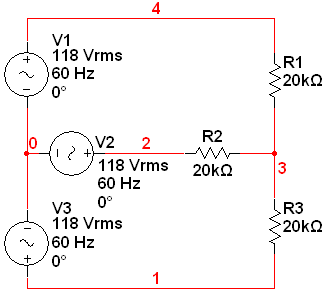
\includegraphics[scale=0.7]{circYY.PNG}
	\caption{Circuito Balanceado $Y-Y$}
	\label{fig1}
\end{figure}
\noindent
Al tener el circuito con carga balanceada se puede decir que la tensión el Nodo $3$ es $0\ V$, lo cual facilita el análisis ya que en cada resistencia $Z_Y$ cae  una tensión de $120\ V_{RMS}$.
\begin{equation}
 {I_a} =\frac {V_{an}}{Z_Y} =\frac {120 \angle 0^\circ V}{ 20 \angle 0^\circ\ K \Omega}= 6\angle 0°\ mA
\label{ecu1}
\end{equation}
\noindent
De igual forma se obtiene  $I_b= 6\angle -120^\circ\ mA$ y $I_c= 6\angle 120^\circ \ mA$.
\begin{equation}
 P = 3  V_f  I_L  cos \theta = 3(120 V)(6 mA)Cos 0^\circ = 2.16\ Watts
\label{ecu2}
\end{equation}
\noindent
Los resultados obtenidos en la simulación fueron:
\begin{table}[H]
	\centering
\begin{tabular}[c]{|c|c|} \hline
$V_{nN}$ & $234.28 \ mV_{rms}$ \\ \hline
$V_{an}$ & $118 \ V_{rms}$ \\ \hline
$V_{ab}$ & $118 \ V_{rms}$ \\ \hline
$V_{cn}$ & $118 \ V_{rms}$ \\ \hline
$V_{ab}$ & $204.398 \ V_{rms}$ \\ \hline
$V_{bc}$ & $204.398 \ V_{rms}$ \\ \hline
$V_{ca}$ & $204.398 \ V_{rms}$ \\ \hline
\end{tabular}
	\caption{Valores obtenidos teóricamente  de los Voltajes}
	\label{tab10}
\end{table}
\begin{table}[H]
	\centering
\begin{tabular}[c]{|c|c|} \hline
$I_{La} = I_{fA}$ & $0.5305\ A_{rms}$ \\ \hline
$I_{Lb} = I_{fB}$ & $0.5299\ A_{rms}$ \\ \hline
$I_{Lc} = I_{fC}$ & $0.5317\ A_{rms}$ \\ \hline
\end{tabular}
	\caption{Valores obtenidos teóricamente  de las Corrientes}
	\label{tab11}
\end{table}
\begin{figure}[H]
	\centering
		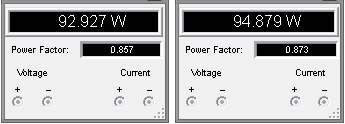
\includegraphics[scale=0.7]{watt1.PNG}
	\caption{Potencia medida en conexión Aron}
	\label{fig10}
\end{figure}
\noindent
Los valores de las resistencias son $R_1 = 220\ \Omega$, $R_2 = 220.5\ \Omega$ y $R_3 = 219\ \Omega$, 3 inductancias de $L = 9\ mH$ con un valor resistivo de $R_L = 2.5\ \Omega$ a una frecuencia de $F = 60\ Hz$.
\begin{figure}[H]
	\centering
		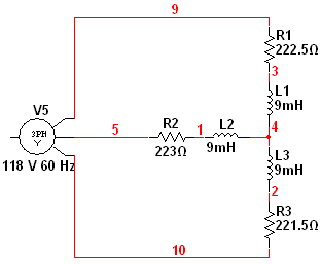
\includegraphics[scale=0.68]{circ1.PNG}
	\caption{Circuito $Y-Y$ rediseñado}
	\label{circ11}
\end{figure}
\noindent
Los resultados obtenidos en la práctica fueron:
\begin{table}[H]
	\centering
\begin{tabular}[c]{|c|c|} \hline
Elemento & Medida \\ \hline
Watimetro1 & $84\ Watts$ \\ \hline
Watimetro2 & $80\ Watts$ \\ \hline
\end{tabular}
	\caption{Valores obtenidos en la práctica de las Potencias}
	\label{tab1}
\end{table}
\begin{table}[H]
	\centering
\begin{tabular}[c]{|c|c|} \hline
$V_{nN}$ & $3.06\ V_{rms}$ \\ \hline
$V_{an}$ & $118.3\ V_{rms}$ \\ \hline
$V_{ab}$ & $119.5\ V_{rms}$ \\ \hline
$V_{cn}$ & $118.6\ V_{rms}$ \\ \hline
$V_{ab}$ & $205.1\ V_{rms}$ \\ \hline
$V_{bc}$ & $205.8\ V_{rms}$ \\ \hline
$V_{ca}$ & $205.3\ V_{rms}$ \\ \hline
\end{tabular}
	\caption{Valores obtenidos en la práctica de los Voltajes}
	\label{tab2}
\end{table}
\begin{table}[H]
	\centering
\begin{tabular}[c]{|c|c|} \hline
$I_{La} = I_{fA}$ & $0.53\ A_{rms}$ \\ \hline
$I_{Lb} = I_{fB}$ & $0.532\ A_{rms}$ \\ \hline
$I_{Lc} = I_{fC}$ & $0.53\ A_{rms}$ \\ \hline
\end{tabular}
	\caption{Valores obtenidos en la práctica de las Corrientes}
	\label{tab3}
\end{table}
\noindent
Las tensiones de línea $V_L$ y de fase $V_f$ obtenidas en la práctica y contenidas en la TABLA \ref{tab2} se aproximan a las obtenidas teóricamente o por simulaciones que se encuentran en la TABLA \ref{tab10}, aunque se puede observar que en la realidad no es posible obtener una fuente trifásica totalmente balanceada.\\
De igual forma las corrientes de línea $I_L$ prácticas de la TABLA \ref{tab3} y teóricas de la TABLA \ref{tab11} son muy cercanas, y que en magnitud tanto teóricas como prácticas no sean iguales se debe a que la carga no es totalmente balanceada.\\
Además, las potencias medidas en la simulación y mostrada en la Fig. \ref{circ11}  se acercan levemente  a las potencias medidas en la parte práctica contenidas en la TABLA \ref{tab1}, debido a que el Wattímetro usado en la práctica no da una medica exacta.

\subsection{Circuito $Y-\Delta$}
\noindent
A continuación se muestra el circuito Y-$\Delta$ con carga balanceada, para este circuito se hace el análisis pertinente.
\begin{figure}[H]
	\centering
		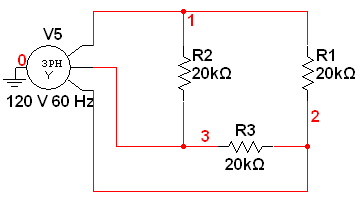
\includegraphics[scale=0.7]{circYD.PNG}
	\caption{Circuito Balanceado $Y-\Delta$}
	\label{fig2}
\end{figure}
\noindent
Nuevamente se tiene un circuito balanceado se facilita el análisis teniendo.
\begin{equation}
 V_L = \sqrt(3)120 \angle \emptyset V =V_{Z\Delta}
 \label{ecu3}
\end{equation}
\noindent
Para esta tensión de línea $V_L$ el ángulo $\emptyset$ cumple el sistema balanceado.
\begin{equation}
 I_L =\frac{V_L}{Z_{\Delta}}=\frac{\sqrt(3)120 \angle \emptyset V}{20 \angle 0^\circ\ K \Omega}=10.392\angle \emptyset mA
 \label{ecu4}
\end{equation}
\noindent
Las corrientes de línea $I_L$, de igual forma tienen ángulos $\emptyset$ balanceados.
\begin{equation}
 P = \sqrt(3)  V_L  I_L  cos \theta
\label{ecu5}
\end{equation}
\begin{equation}
 P =\sqrt(3)(\sqrt(3)120 V)(10.392 mA)cos 0^\circ = 3.741\ Watts
\label{ecu6}
\end{equation}
\noindent
Los resultados obtenidos en la simulación fueron:
\begin{table}[H]
	\centering
\begin{tabular}[c]{|c|c|} \hline
$V_{nN}$ & $234.28 \ mV_{rms}$ \\ \hline
$V_{an}$ & $118 \ V_{rms}$ \\ \hline
$V_{ab}$ & $118 \ V_{rms}$ \\ \hline
$V_{cn}$ & $118 \ V_{rms}$ \\ \hline
$V_{ab}$ & $204.398 \ V_{rms}$ \\ \hline
$V_{bc}$ & $204.398 \ V_{rms}$ \\ \hline
$V_{ca}$ & $204.398 \ V_{rms}$ \\ \hline
\end{tabular}
	\caption{Valores obtenidos teóricamente  de los Voltajes}
	\label{tab12}
\end{table}
\begin{table}[H]
	\centering
\begin{tabular}[c]{|c|c|} \hline
$I_{La}$ & $1.589 \ A_{rms}$ \\ \hline
$I_{Lb}$ & $1.539\ A_{rms}$ \\ \hline
$I_{Lc}$ & $1.595\ A_{rms}$ \\ \hline
$I_{FA}$ & $0.918\ A_{rms}$ \\ \hline
$I_{FB}$ & $0.916\ A_{rms}$ \\ \hline
$I_{FC}$ & $0.922\ A_{rms}$ \\ \hline
\end{tabular}
	\caption{Valores obtenidos teóricamente de las Corrientes}
	\label{tab13}
\end{table}
\begin{figure}[H]
	\centering
		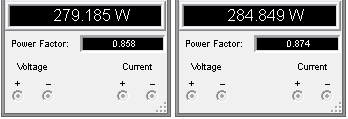
\includegraphics[scale=0.7]{watt2.PNG}
	\caption{Potencia medida en conexión Aron}
	\label{fig12}
\end{figure}
\noindent
Los valores de las resistencias son $R_1 = 220\ \Omega$, $R_2 = 220.5\ \Omega$ y $R_3 = 219\ \Omega$, 3 inductancias de $L = 9\ mH$ con un valor resistivo de $R_L = 2.5\ \Omega$ a una frecuencia de $F = 60\ Hz$.
\begin{figure}[H]
	\centering
		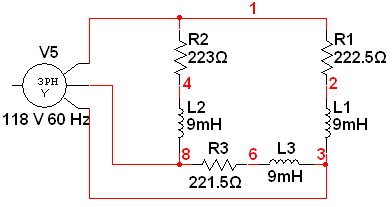
\includegraphics[scale=0.65]{circ2.PNG}
	\caption{Circuito $Y-\Delta$ rediseñado}
	\label{circ13}
\end{figure}
\noindent
Los resultados obtenidos en la práctica fueron:
\begin{table}[H]
	\centering
\begin{tabular}[c]{|c|c|} \hline
Elemento & Medida \\ \hline
Watímetro 1 & $122\ Watts$ \\ \hline
Watímetro 2 & $134\ Watts$ \\ \hline
\end{tabular}
	\caption{Valores obtenidos en la práctica de las Potencias}
	\label{tab4}
\end{table}
\begin{table}[H]
	\centering
\begin{tabular}[c]{|c|c|} \hline
$V_{an}$ & $118.3\ V_{rms}$ \\ \hline
$V_{ab}$ & $119.5\ V_{rms}$ \\ \hline
$V_{cn}$ & $118.6\ V_{rms}$ \\ \hline
$V_{ab}$ & $205.1\ V_{rms}$ \\ \hline
$V_{bc}$ & $205.8\ V_{rms}$ \\ \hline
$V_{ca}$ & $205.3\ V_{rms}$ \\ \hline
\end{tabular}
	\caption{Valores obtenidos en la práctica de los Voltajes}
	\label{tab5}
\end{table}
\begin{table}[H]
	\centering
\begin{tabular}[c]{|c|c|} \hline
$I_{La}$ & $1.363\ A_{rms}$ \\ \hline
$I_{Lb}$ & $1.367\ A_{rms}$ \\ \hline
$I_{Lc}$ & $1.366\ A_{rms}$ \\ \hline
$I_{FA}$ & $0.458\ A_{rms}$ \\ \hline
$I_{FB}$ & $0.456\ A_{rms}$ \\ \hline
$I_{FC}$ & $0.903\ A_{rms}$ \\ \hline
\end{tabular}
	\caption{Valores obtenidos en la práctica de las Corrientes}
	\label{tab6}
\end{table}
\noindent
Las tensiones de línea $V_L$ y de fase $V_f$ tanto teóricos como prácticos se comporta igual a las tensiones medidas en el circuito $Y-Y$.\\
Se puede observar que las corrientes de línea $I_L$ medidas teóricamente  consignadas en la TABLA \ref{tab13} y las obtenidas en la práctica y contenidas en la TABLA \ref{tab6} son aproximadamente iguales, mientras que las corrientes de fase $I_F$  son diferentes notablemente excepto la corriente $I_{FC}$ la cual es aproximadamente igual, esto tal vez se da por un error en la medida  o en el montaje del circuito al momento de medir estas corrientes, o al el hecho de que la carga no es totalmente balanceada.\\
Para la medición de la potencia en conexión Aron se puede comparar los datos teóricos de la Fig. \ref{fig12} y los datos obtenidos en la práctica contenidos en la TABLA\ref{tab4} , los datos son notablemente diferentes, esto puede deberse a error  en el momento de la conexión además que los Wattímetros usados en la practica no son elementos de medida exactos.

\subsection{Rectificación de media Onda}
\noindent
En esta parte de la práctica se diseña un circuito con una fuente trifásica, luego se aplica un rectificador de media onda en cada señal, la salida de cada fase se suma para obtenerla señal que se aplicara a la carga.\\
Los datos obtenidos teóricamente o a través de simulaciones son:
\begin{figure}[H]
	\centering
		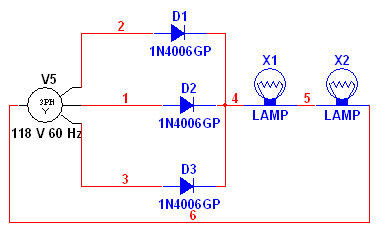
\includegraphics[scale=0.7]{circ3.PNG}
	\caption{Circuito rectificador de media onda trifásico}
	\label{circ14}
\end{figure}
\begin{figure}[H]
	\centering
		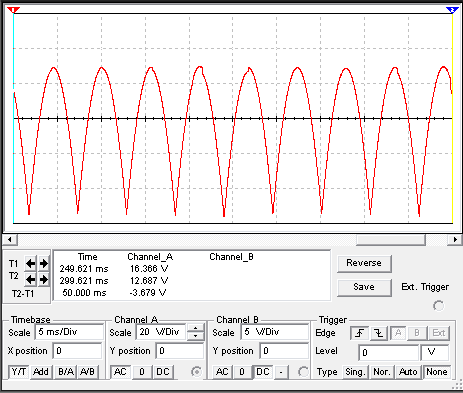
\includegraphics[scale=0.5]{onda.PNG}
	\caption{Onda obtenida en la rectificación simulada}
	\label{fig15}
\end{figure}
\begin{table}[H]
	\centering
\begin{tabular}[c]{|c|c|} \hline
$V_{carga_{DC}}$ & $137.053\ V$ \\ \hline
$V_{carga_{AC}}$ & $25.194\ V_{rms}$ \\ \hline
\end{tabular}
	\caption{Valores obtenidos a través de simulaciones de los Voltajes}
	\label{tab81}
\end{table}
\noindent
Los demás datos como corrientes de línea  $I_L$ y potencia no se pueden obtener a partir de simulaciones, ya que no es posible simular una bombilla de $100\ watts$.\\
Los resultados obtenidos en la práctica fueron:
\begin{table}[H]
	\centering
\begin{tabular}[c]{|c|c|} \hline
Elemento & Medida \\ \hline
Watímetro 1 & $43\ Watts$ \\ \hline
Watímetro 2 & $43\ Watts$ \\ \hline
\end{tabular}
	\caption{Valores obtenidos en la práctica de las Potencias}
	\label{tab7}
\end{table}
\begin{table}[H]
	\centering
\begin{tabular}[c]{|c|c|} \hline
$V_{carga_{DC}}$ & $138.6\ V$ \\ \hline
$V_{carga_{AC}}$ & $35.11\ V_{rms}$ \\ \hline
\end{tabular}
	\caption{Valores obtenidos en la práctica de los Voltajes}
	\label{tab8}
\end{table}
\begin{table}[H]
	\centering
\begin{tabular}[c]{|c|c|} \hline
$I_{L_{DC}}$ & $0.632\ A$ \\ \hline
$I_{{LA}_{AC}}$ & $0.304\ A_{rms}$ \\ \hline
$I_{{LB}_{AC}}$ & $0.309\ A_{rms}$ \\ \hline
$I_{{LC}_{AC}}$ & $0.309\ A_{rms}$ \\ \hline
$I_{carga_{AC}}$ & $0.116\ A_{rms}$ \\ \hline
\end{tabular}
	\caption{Valores obtenidos en la práctica de las Corrientes}
	\label{tab9}
\end{table}
\noindent
El tiempo que se utilizo para calcular la potencia consumida por medio del contador fue de $t=8.4\ min$ para $0.1\ Kw-H$, la energía calculada con este tiempo y el valor obtenido con los Wattimetros es $E_t = 0.01204\ Kw-H$, estos valores deberían dar aproximadamente iguales, se desconoce el porque estos valores difieren tanto, esto puede ser ocasionado por que el contador trifásico se encontraba descalibrado, o se genero un error al medir dicha energía (Error de escala o de manipulación del elemento).
\begin{figure}[H]
 \centering
    \subfigure[Imagen del Contador Trifásico]{\label{figa}
      \fbox{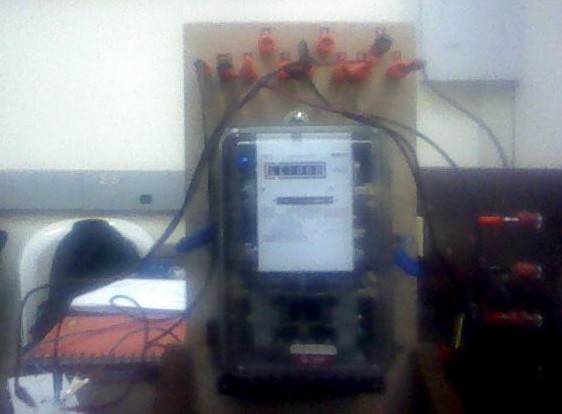
\includegraphics[scale=0.44]{001.png}}}
  \hspace{2cm}
    \subfigure[Imagen del Contador Trifásico y del montaje]{\label{figb}
      \fbox{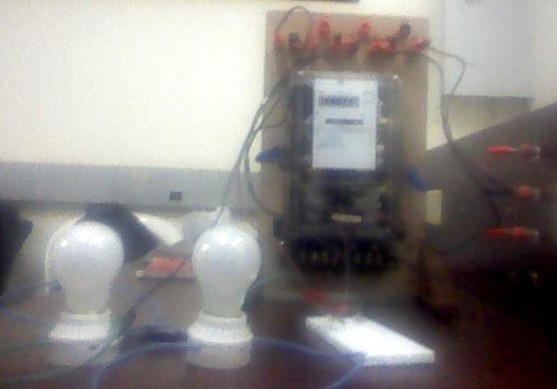
\includegraphics[scale=0.44]{011.png}}}
  \caption{Imagenes del montaje con el Contador Trifásico}
    \label{fig7}
\end{figure}
\noindent
Al comparar los datos obtenidos en simulaciones de la TABLA \ref{tab81} y los datos obtenidos en la práctica contenidos en la TABLA \ref{tab8} se puede observar que tanto en $DC$ como en $AC$ son aproximadamente iguales y se obtienen de la señal mostrada en la Fig. \ref{fig15}.

\section{Conclusiones}
\begin{itemize}
 \item Se comprobó de manera empírica que para saber la potencia consumida por una carga trifásica, sin importar si esta es balanceada o no, se puede hacer a partir de dos Watimetros utilizando la conexión Aron.
 \item En la realidad no se puede obtener una carga balanceada o una fuente trifásica balanceada debido corrientes parásitas, variación de las resistencias, campos magnéticos, entre otros.
 \item Al rectificar la señal trifásica y sumarla como se explico anteriormente, esta de igual forma esta entregando una energía a la carga conectada, en este caso dos bombillas, debido a esto las bombillas se enciende.
 \item Se comprobó que las tensiones de linea $V_L$ y de fase $V_f$ se mantienen constantes sin importar la carga que se conecte a la fuente trifásica.
 \item Cuando se presenta un pequeño desbalance en una carga conectada en $\Delta$, existe una pequeña variación en los voltajes de linea, pero la variación de las corrientes de fase es notorio, esto se vio en la practica al medir las corrientes del circuito Y-$\Delta$.
\end{itemize}

\begin{figure}[H]
	\centering
		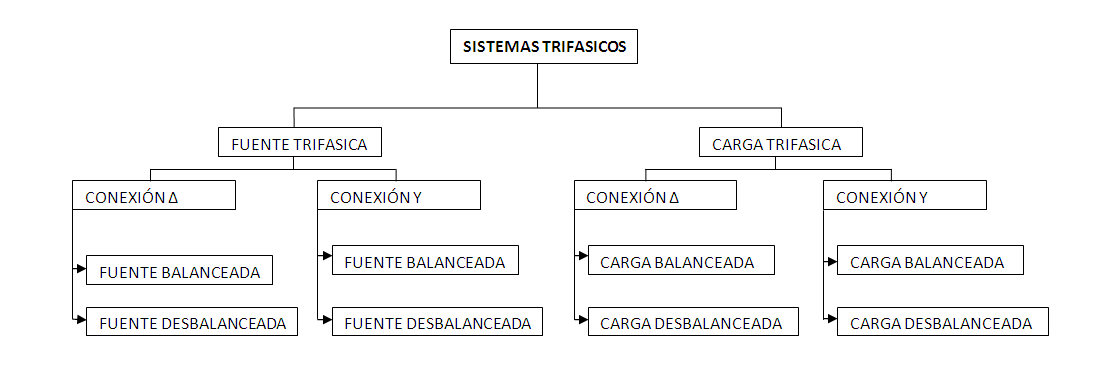
\includegraphics[scale=0.63]{mapa.png}
	\caption{Mapa conceptual de los Sistema Trifásicos}
	\label{figura12}
\end{figure}

\bibliographystyle{ieeetran}
\begin{thebibliography}{99}
\bibitem{sadiku} Alexander, Charles K. \&  Sadiku, Matthew N.O.
{\em ```Fundamentals of Electric Circuits"'}.
McGRAW-HILL, ISE Editions, 1999.

\bibitem{dorf} Dorf  \& Svoboda.
{\em ```Circuitos Eléctricos"'}.
Alfaomega, Sexta Edición, 2006.

\bibitem{hayt} Hayt, William H. Jr., Kemmerly, Jack E. \& Durbin, Steven M.
{\em ```Análisis de circuitos en ingeniería"'}.
McGRAW-HILL, Séptima Edición, 2007.

\bibitem{nahvi} Nahvi, Mahmood \& Edminister, Joseph A.
{\em ```Theory and Problems of Electric Circuits"'}.
McGRAW-HILL, Fourth Edition, 2003.

\end{thebibliography}
\end{document}